%!TEX program = xelatex

\documentclass[a4paper,UTF8]{ctexart}
\usepackage{amsmath}
\usepackage{amssymb}
\usepackage{changepage}
\usepackage{pgf}
\usepackage{tikz}
\usepackage{multicol}
\usetikzlibrary{arrows,automata}
% \usepackage[latin1]{inputenc}
\usepackage{verbatim}

\newcommand{\pro}[2]{\boldsymbol{#1} \rightarrow \boldsymbol{#2}}
\newcommand{\apro}[2]{\boldsymbol{#1} &\rightarrow \boldsymbol{#2}}

 \newcommand{\goto}{\vdash}
 \newcommand{\set}[1]{\{ #1 \}}
 \newcommand{\trans}[2]{\delta(#1)=(#2)}
\usepackage[margin=1.25in]{geometry}
\usepackage{color}
\usepackage{graphicx}
\usepackage{amssymb}
\usepackage{amsmath}
\usepackage{amsthm}
\usepackage{multirow}
\usepackage{pdfpages}
\usepackage{fontspec}                   % requires XeLaTeX

\theoremstyle{definition}
\newtheorem*{solution}{Solution}
\newtheorem*{prove}{Proof} 

\setmainfont                    [Ligatures=TeX]{Times New Roman}
\parindent=0pt 
\topskip=-200pt

\begin{document} 
\title{PTC (Fall 2018) -- Assignment 2}
\author{徐翔哲}
\maketitle
\newpage

\section*{Problem 1}
Give context free grammars that generate the following languages, and give a brief description of the functionality of each variable in your grammars (in natural language).
\begin{enumerate}
	\item[a.] \{$w\in \{a,b\}^*\ |\mbox{ the number of $a$'s in $w$ is more than the number of $b$'s in $w$}$\}
	\item[b.] \{$a^ib^{2j}c^{j}d^{k}\ |\ i,j,k\geq 1, k \geq 2i$\}
	\item[c.] \{$w\in \{a,b\}^*\ |\ abb\mbox{ and }aab\mbox{ are substrings of }w$\}
	\item[d.] \{$a^{i}b^{j}c^{k}\ |\ i,j,k\geq 0 \wedge i + j > k$\}
\end{enumerate}

\subsection*{a}
It can be proved that for all string w having $n$ more $a$ than $b$,
it can be divided into $n$ substrings, say $w_0w_1w_2...$. For  each $w_i$
the number of $a$ is exactly one more the number of $b$.

\begin{alignat*}{2}
	\apro{S}{AS|A}           \\
	\apro{A}{a|aB|bAA}       \\
	\apro{B}{aC|bA|\epsilon} \\
	\apro{C}{bB|aCC|b}
\end{alignat*}

$A$ is the language where $\#a=\#b+1$, $B$ is the language where $\#a=\#b$, $C$ is the language where $\#b=\#a+1$.

\subsection*{b}
\begin{alignat*}{2}
	\apro{S}{aTdd}      \\
	\apro{T}{aTdd|Td|B} \\
	\apro{B}{bbc|bbBc}
\end{alignat*}

The functionality of the variables are clear.

\subsection*{c}
\begin{alignat*}{2}
	\apro{S}{aS|bS|Sa|Sb|T|aabb} \\
	\apro{T}{UV|VU}              \\
	\apro{U}{aU|bU|Ua|Ub|aab}    \\
	\apro{V}{aV|bV|Va|Vb|abb}
\end{alignat*}

$U$ means the language whose substring contains $aab$,
$V$ means the language whose substring contains $abb$.
And $T$ means the language having $aab$ and $abb$ as substrings separately.
Finally, consider one special case $S$, where the string contains $aabb$, which also has both
$aab$ and $abb$ as substrings.

\subsection*{d}

\begin{alignat*}{2}
	\apro{S}{aA|bB}           \\
	\apro{A}{aAc|aA|B}        \\
	\apro{B}{bB|bBc|\epsilon}
\end{alignat*}

The main idea is that for every $c$ in this language, there exists one related $a$ or $b$. Also, 
since the number of $a$ or $b$ is strictly larger than the number of $c$, we can infer that for all the 
string in this language, there's at least one $a$ or one $b$ before any $c$ is generated.
\section*{Problem 2}
Consider the following CFG $G$:
\[
	\begin{aligned}
		S & \rightarrow SS\ |\ T   \\
		T & \rightarrow aTb\ |\ ab
	\end{aligned}
\]
Describe $L(G)$ and show that $G$ is ambiguous. Give an unambiguous grammar $H$
where $L(H) = L(G)$ and sketch a proof that $H$ is unambiguous.
\\

$L(G)$ = $\{a^ib^i|i\geq 1\}^+$
Consider the string $ababab$. There exists two different derivation trees.

\begin{multicols}{2}
	
	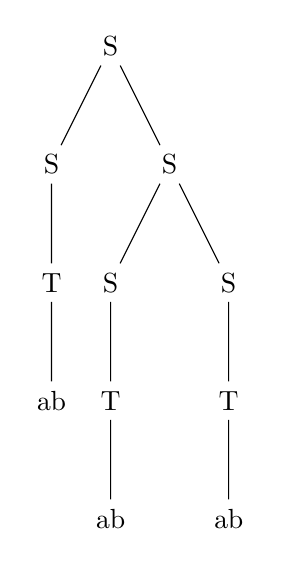
\begin{tikzpicture}
		\node {S}
		child {node {S}
				child{node{T}
						child{node{ab}}}}
		child {node {S}
				child {node {S}
						child{node{T}
								child{node{ab}}}}
				child {node {S}
						child{node{T}
								child{node{ab}}}}}
		;
	\end{tikzpicture}
	
	
	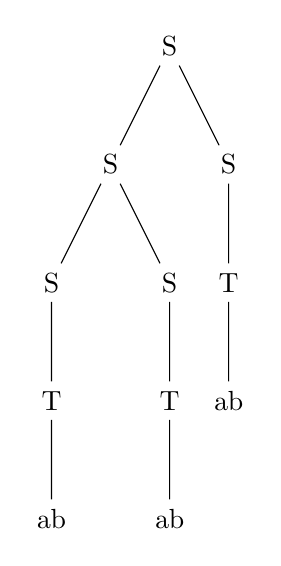
\begin{tikzpicture}
		\node {S}
		child {node {S}
				child {node {S}
						child{node{T}
								child{node{ab}}}}
				child {node {S}
						child{node{T}
								child{node{ab}}}}}
		child {node {S}
				child{node{T}
						child{node{ab}}}}
		;
	\end{tikzpicture}
\end{multicols}

Define grammar $H$ as follows:
\begin{alignat*}{2}
	\apro{S}{ST|T}   \\
	\apro{T}{aTb|ab}
\end{alignat*}
Use structural induction:
\begin{itemize}
	\item $\pro{T}{aTb|ab}$ is obvious unambiguous
	\item $\pro{S}{T}$ is obvious unambiguous
	\item $\pro{S}{ST}$:The variable S can only be generated on the left side of T, so for
	      a serial of T, the only way to derivate it will be $\pro{S}{\pro{ST}{(ST)T}}$. So this constructor is 
	      unambiguous.
\end{itemize}
Up to now, we have proved that every production of $H$ is unambiguous, so $H$ is unambiguous. 

\section*{Problem 3}
Let $G = (V, T, P, S)$ be a context free grammar such that $V = \{A, B\}$, $T = \{a, b\}$, $S = B$ and $P$ is
\[
	\begin{aligned}
		B & \rightarrow aAA              \\
		A & \rightarrow aB \ |\ bB\ |\ a
	\end{aligned}
\]
\begin{enumerate}
	\item[a.] Give parse trees, leftmost and rightmost derivations for the following strings.
	      \begin{itemize}
		      \item[1.] $aabaaa$
		      \item[2.] $abaaabaaa$
	      \end{itemize}
	\item[b.] Convert $G$ to a PDA that accepts the same language by empty stack.
\end{enumerate}

\subsection*{a}
\subsubsection*{1}

\begin{multicols}{2}
	
	\begin{tikzpicture}
		\node {B}
		child {node {a}}
		child {node {A}
				child{node{a}}}
		child {node{A}
				child{node{b}}
				child{node{B}
						child{node{a}}
						child{node{A}
								child{node{a}}}
						child{node{A}
								child{node{a}}}}}
		;
	\end{tikzpicture}
	
	rightmost: $B\Rightarrow aAA \Rightarrow aAbB \Rightarrow aAbaAA \Rightarrow aAbaAa \Rightarrow aAbaaa \Rightarrow aabaaa$
	
	leftmost: $B \Rightarrow aAA \Rightarrow aaA \Rightarrow aabB \Rightarrow aabaAA \Rightarrow aabaaA \Rightarrow aabaaa$
	
\end{multicols}


\subsubsection*{2}
	\begin{tikzpicture}
		\node {B}
		child {node {a}}
		child {node {A}
				child{node{b}}
				child{node{B}
						child{node{a}}
						child{node{A}
								child{node{a}}}
						child{node{A}
                child{node{a}}}}}
    child[missing]
		child {node{A}
        child{node{b}}
        child[missing]        
				child{node{B}
						child{node{a}}
						child{node{A}
								child{node{a}}}
						child{node{A}
								child{node{a}}}}}
		;
	\end{tikzpicture}
	
  rightmost: $B\Rightarrow aAA \Rightarrow aAbB \Rightarrow aAbaAA \Rightarrow aAbaAa
  \Rightarrow aAbaaa \Rightarrow abBbaaa \Rightarrow abaAAbaaa \Rightarrow abaAabaaa \Rightarrow abaaabaaa$
	
  leftmost: $B \Rightarrow aAA \Rightarrow abBA \Rightarrow abaAAA \Rightarrow abaaAA 
  \Rightarrow abaaaA \Rightarrow abaaabB \Rightarrow abaaabaAA \Rightarrow abaaabaaA \Rightarrow abaaabaaa $
	
\subsection*{b}
\[PDA\ P=(Q,q_0,\Sigma,\Gamma,Z_0,\delta)\]
\[Q=\{q_0\} \]
\[\Sigma = \{a,b\}\]
\[\Gamma = \{A,B,S\} \cup \Sigma\]  
\[Z_0 = S\]
\newcommand{\f}[2]{\delta(#1) &\rightarrow (#2)}
\begin{alignat*}{2}
  \f{q_0,\epsilon,S}{q_0,B}\\
  \f{q_0,\epsilon,B}{q_0,aAA}\\
  \f{q_0,\epsilon,A}{q_0,aB}\\
  \f{q_0,\epsilon,A}{q_0,bB}\\
  \f{q_0,\epsilon,A}{q_0,a}\\
  \f{q_0,a,a}{q_0,\epsilon}\\
  \f{q_0,b,b}{q_0,\epsilon}\\
\end{alignat*}


\section*{Problem 4}
Begin with the grammar:
\[
	\begin{aligned}
		S & \rightarrow aAa\ |\ bBb\ |\ \epsilon \\
		A & \rightarrow C \ |\ a                 \\
		B & \rightarrow C \ |\ b                 \\
		C & \rightarrow CDE\ |\ \epsilon         \\
		D & \rightarrow A\ |\ B\ |\ ab
	\end{aligned}
\]
\begin{enumerate}
	\item[a.] Eliminate $\epsilon$-productions.
	\item[b.] Eliminate any unit productions in the resulting grammar of (a.).
	\item[c.] Eliminate any useless symbols in the resulting grammar of (b.).
	\item[d.] Put the resulting grammar of (c.) into Chomsky normal form.
\end{enumerate}

\subsection*{a}
The nullable variables are $C,S,A,B,D$, then we can get:
\begin{alignat*}{2}
  \apro{S}{aAa|bBb|aa|bb}\\
  \apro{A}{C|a}\\
  \apro{B}{C|b}\\
  \apro{C}{CDE|CE|DE|E}\\
  \apro{D}{ab|A|B}
\end{alignat*}

\subsection*{b}

\begin{alignat*}{2}
  \apro{S}{aAa|bBb|aa|bb}\\
  \apro{A}{CDE|CE|DE|E|a}\\
  \apro{B}{CDE|CE|DE|E|b}\\
  \apro{C}{CDE|CE|DE|E}\\
  \apro{D}{ab|CDE|CE|DE|E|a|CDE|CE|DE|E|b}
\end{alignat*}

\subsection*{c}
\begin{alignat*}{2}
  \apro{S}{aAa|bBb|aa|bb}\\
  \apro{A}{a}\\
  \apro{B}{b}\\
\end{alignat*}

\subsection*{d}
\begin{alignat*}{2}
  \apro{S}{AT_1|BT_2|AA|BB}\\
  \apro{T_1}{AA}\\
  \apro{T_2}{BB}\\  
  \apro{A}{a}\\
  \apro{B}{b}\\
\end{alignat*}

\section*{Problem 5}
Given grammar $G$:
\[
	\begin{aligned}
		S & \rightarrow AB\ |\ BC \\
		A & \rightarrow BA\ |\ a  \\
		B & \rightarrow CC\ |\ b  \\
		C & \rightarrow AB\ |\ a
	\end{aligned}
\]
Please use CYK algorithm to decide whether string $ababa$ belongs to $L(G)$.
\newcommand{\cyk}[3]{ababa[#1:#2]:\{#3\}\\}\\
\cyk{0}{0}{A,C}
\cyk{1}{1}{B}
\cyk{2}{2}{A,C}
\cyk{3}{3}{B}
\cyk{4}{4}{A,C}
\cyk{0}{1}{S,C}
\cyk{1}{2}{A,S}
\cyk{2}{3}{S,C}
\cyk{3}{4}{A,S}
\cyk{0}{2}{B}
\cyk{1}{3}{S,C}
\cyk{2}{4}{B}
\cyk{0}{3}{B}
\cyk{1}{4}{B}
\cyk{0}{4}{S}
Since $ababa[0:4]$ contains $S$, this string belongs to $L(G)$

\section*{Problem 6}
Use the CFL pumping lemma to show each of these languages are not context free.
\begin{enumerate}
	\item[a.] $\{a^ib^jc^k\ |\ i < j < k\}$
	\item[b.] $\{0^p\ |\ p\mbox{ is a prime}\}$
	\item[c.] $\{ww^Rw\ |\ w \in \{0,1\}^* \}$
\end{enumerate}

\subsection*{a}

$\forall n$, choose $a^nb^(n+1)c^(n+2)$. Since $|vwx|\leq n$, so 
$|vx|$ contains at least one of character $a$, $b$ and $c$ but not all.\\
If $vx$ doesn't contain $c$, we repeat $vx$ for $2n$ times. In such case, the number
of a or b is larger than the number of c.\\
If $vx$ contains $c$, then it cannot contain $a$. Then we remove $vx$ from the origin string,
which will cause either the number of b is not larger than the number of a or
the number of c is not larger than the number of b.

\subsection*{b}
Suppose that $|vx|=q$, then we repeat $|vx|$ for $p+1$ times.
Then $|uv^{p+1}wx^{p+1}y|=p+p\cdot q =(1+q)p $, which is not a prime. So $uv^{p+1}wx^{p+1}y$ is not in this language.

\subsection*{c}
Let $|w|>n$, also, choose $w$ such that every w's prefix is not w's suffix. 
Since $|vwx|<n$, so $|vx|$ can't contain both the beginning and the ending of w.
Suppose that uwy=wab, where a isi one prefix of $w^R$ and b is one suffix of w.
If wab can be written as $ss^Rs$, it should be one of the following case:
\begin{figure}[!h]
  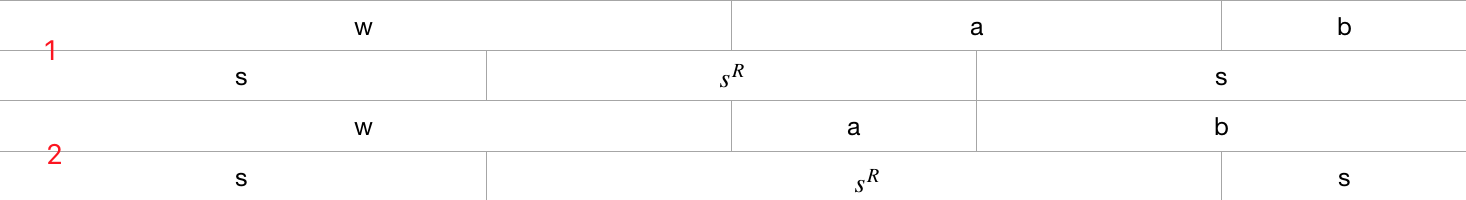
\includegraphics[width=0.8\textwidth]{ssr.png}
\end{figure}\\
case1 means suffix($s^R$)=prefix(a) $\Rightarrow$ suffix($w^R$)=prefix($w^R$)
$\Rightarrow$ prefix(w)=suffix(w), which is a contradiction with our hypothesis.

case2 means w's suffix being w's prefix, which is a contradiction with our hypothesis.




\section*{Problem 7}
Show that the CFL is closed under the following operations:
\begin{enumerate}
	\item[a.] $init(L)=\{w\ |\mbox{ for some }x, wx \in L\}$. (\textbf{Hint}: Start with a CNF grammar for the language $L$)
	\item[b.] $cycle(L)=\{xy\ |\ yx \in L\}$ (\textbf{Hint}: Try a PDA-based construction)
\end{enumerate}

\subsection*{a}

For all the production: 

If $\pro{P}{\alpha}$, convert it to $\pro{P'}{\alpha|\epsilon}$;\\
if $\pro{P}{AB}$, convert it to $\pro{P'}{AB'|A'}$

Proof:
Induction on the steps of derivation. 

Basis: $\pro{P}{\alpha}$, the $P'$ is all the prefix of $\alpha$($\alpha$ and $\epsilon$) .

Induction:
	For all derivation within n step, the new grammar will generate all the prefix
	of the strings that can be derived within n steps. 

	For the derivation of step n+1, we first make one step.\\
	If the first step is $\pro{P'}{AB'}$, then $B'$ contains all the prefix of B since it
	can be derived within n steps. Then we can get that $P'$ contains all the 
	prefix of P.\\
	If the first step is $\pro{P'}{A'}$, then $A'$ contains all the prefix of 
	$A$ since it can be derived within n steps. Then we can get that $P'$ contains all
	the prefix of P.

	Now we have proved that all the strings the new grammar generate are the prefix of strings 
	in the origin language.

\subsection*{b}


\section*{Problem 8}
If $L$ is regular, it satisfies pumping lemma for sure! But if a language satisfies pumping lemma, is it regular? Prove or disprove it.

$(abc)^+0^n1^n$, choose n=4, and let $x=\epsilon,\ y=abc$. However, this language is obviously not 
a regular language.



\end{document}
